\section{Methodology}
First of all, I have studied the current industrial landscape and the challenges faced in the use of robotic arms sothat I can find the best way to design my robotic arm. 
 I have Identified the specific tasks that the proposed robotic arm must perform. The robot can be used in many sector in our daily activities. The robot can be used in medical sector, engineering sector for simplify our tasks. This robot can carry 40 kg of weight easily. Development of a set of specifications and constraints for the robotic arm has been done. I have Analysed the existing solutions and technologies available in the market for my robotic arms. Because if the materials needed for creating the robot are not available in markets then it will impossible to handle the project.\\ 
 \begin{figure}[h]
    \centering
    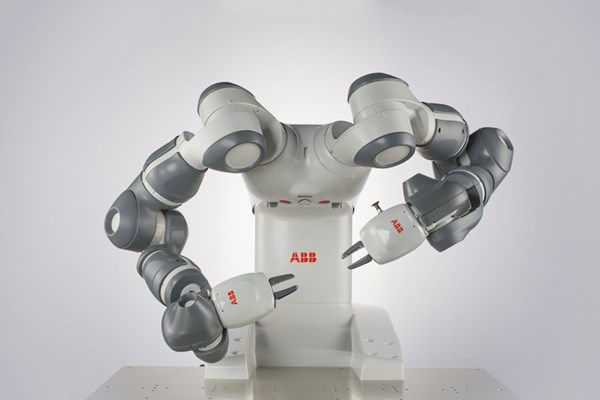
\includegraphics[width = .85\linewidth]{pic/2.jpeg}
    \caption{Designed arm robot}
    \label{fig:fig3}
\end{figure}
 Second of all, The task that is needed for creating robot is design plan of robotic arms. After studying a lot about the existing robot I decided to create the robot.
 Then all the components needed for creating the robot are purchased. I have created a 3D models and simulations to evaluate the design and performance of the robotic arms and optimized the design for reliability and efficiency. The design I have selected for my project is shown in figure~\ref{fig:fig3}.\\
Third of all, the robot I have designed can be divided in two main part. One is mechanical part design and other part is electrical part design. For mechanical part design there are many component are needed such as motor. Mechanical part is basically used for movement of arm top-bottom, left-right and rotation. Other part is electrical part. This part is used for supplying power for the robot.  For the movement of the robot and activating the motor used inside the robot electricity is needed. Different types of wire are used for proper robot making. I have used color with awesome combination. Some algorithms are used for interact hardware and software used for the robot. I have Finalized of the design and fabrication of the robotic arm with taking long times. This robot needs integration control system with other systems and development of a user-friendly interface for the control system. \\ 
 Finally robot is tested whether it works successfully. The robot has two arms. The robot can be used in many sector in our daily activities. The robot can be used in medical sector, engineering sector for simplify our tasks. This robot can carry 40 kg of weight easily.\\
 This methodology outlines the steps and processes that will be followed to design, develop, and deploy the proposed multi-purpose robotic arm. The methodology takes into account the requirements gathering, design and optimization, prototyping and testing, control system development, implementation and deployment, and maintenance and upgrades. The methodology is designed to ensure the achievement of the objectives and expected outcomes of the project.



